\section{Background}

This section provides a brief overview of the technologies and techniques used in our approach. We discuss the instance segmentation task on images, the DynamicEdgeConv Graph Neural Network, Octree algorithm for reducing points, and the SMOTE technique to address class imbalance. Although we explored Siamese networks, they were not included in the final solution.

\subsection{Instance Segmentation task on images, and how it is analogous to our problem} \label{ssec:intseg}

    \begin{figure}
        \centering
        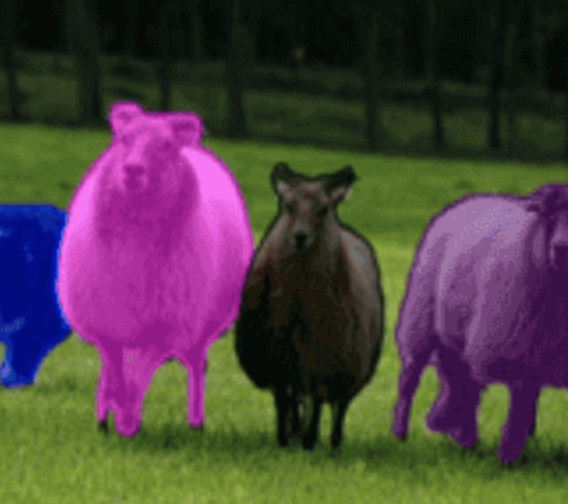
\includegraphics[width=0.75\linewidth]{images/instance_seg_example.png}
        \caption{Instance Segmentation Example from~\cite{intsegimg}: here we can see in this image how the pixels containing the sheep are differentiated from the background and also each sheep is coloured with different hues. Thus the model not only classifies each pixel into one of the classes, but also tells which sheep that pixel belongs to.}
        \label{fig:intseg}
    \end{figure}

    Instance segmentation is a computer vision task that deals with detecting, classifying, and segmenting individual objects within an image. This technique assigns unique labels to each object instance in the scene, enabling pixel-wise mask generation for each distinct object. In other words, instance segmentation not only identifies the classes of objects present in an image but also distinguishes between different instances of the same class as shown in Figure \ref{fig:intseg}.

    In our problem, we focus on substructure-finding in dark matter halos from gravity-only N-body simulations using point cloud segmentation techniques based on Graph Neural Network (GNN) methods. Here, each particle can be either labeled as background (meaning it is not a part of any subhalo) or classified as a part of one of the subhalos.

    The instance segmentation task on images and our point cloud classification problem share similarities in their goals: both tasks aim to classify individual elements within their respective data types (pixels for images, particles for point clouds) into distinct classes and instances. By applying instance segmentation concepts from image processing, we can identify and separate individual subhalos within the point cloud before classifying them, potentially improving classification performance by allowing for more focused analysis of each object in the scene.

    Instance segmentation on images involves classifying and differentiating between instances of objects at the pixel level. In our problem, we apply similar concepts to point clouds, where particles are classified into distinct classes and instances, enabling improved substructure-finding within dark matter halos from gravity-only N-body simulations.0


\subsection{Octree}\label{ssec:octree}


    \begin{figure}
        \centering
        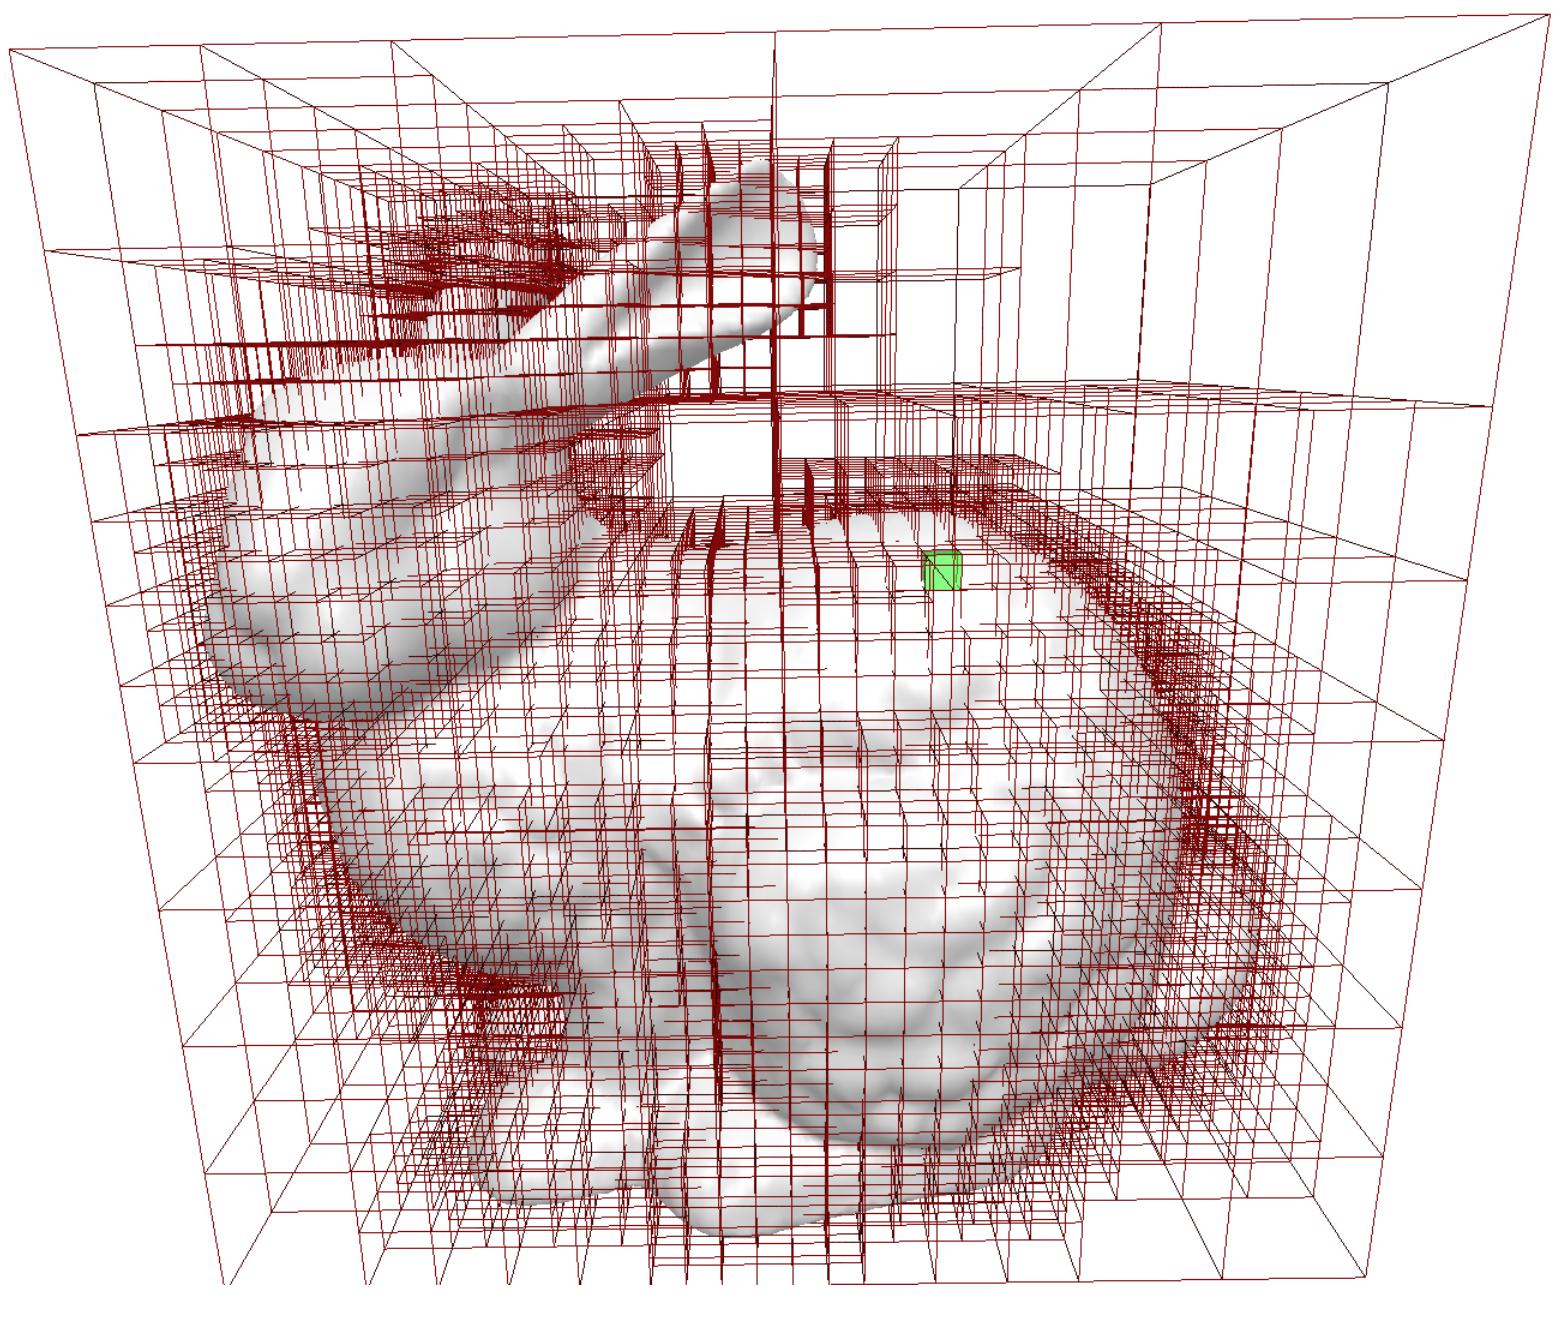
\includegraphics[width=0.75\linewidth]{images/octree.png}
        \caption{Octree Representation of a model of a rabbit taken from~\cite{octree}. Here we can see how the voxels become smaller and smaller as it reaches closer to the surface of the model, and becomes large away from the model surface}
        \label{fig:octree}
    \end{figure}

    The Octree algorithm is a hierarchical spatial partitioning technique used to efficiently manage and process large datasets, particularly those with varying densities. In our case, we aim to reduce the number of points in our point cloud data, which will help optimize both time and memory usage.
    
    Initially, we could have divided the space into grids, treating all points inside a single cube (voxel) as a single point. This approach would have introduced a new features for each voxel: mass, equal to the number of points within that voxel. We also recalculate the position and the velocities, as the mean of all points in that voxel.
    
    However, our dataset presents a challenge due to its varying density. Some regions are extremely dense, while others are extremely sparse. A naive grid-based approach would be wasteful, as many voxels would remain empty, while others would contain an overwhelming number of points. To address this issue, we employ the Octree algorithm. We can see in Figure \ref{fig:octree} how we use different sizes of voxels all over the grid.
    
    The Octree algorithm is a recursive partitioning method that adaptively subdivides the 3D space into smaller regions based on the density of points within each region. This approach ensures that dense regions are divided into smaller voxels, while sparse regions are covered by larger voxels, thereby optimizing memory and computational resources.
    
    Here's a step-by-step explanation of the Octree algorithm:
    
    \begin{enumerate}
        \item \textbf{Root Node Creation:} The algorithm begins with the creation of a root node, which represents the entire 3D space.
        \item \textbf{Point Insertion:} Each point in the dataset is inserted into the Octree by recursively traversing the tree. At each node, the point is directed to one of eight possible child nodes based on its spatial location (e.g., top-left-front, bottom-right-rear, etc.).
        \item \textbf{Node Splitting:} When a node exceeds a predetermined capacity (i.e., the maximum number of points it can hold), it is split into eight smaller child nodes. This process continues recursively until each node meets the capacity constraint or the minimum voxel dimensions is reached.
        \item \textbf{Voxel Creation:} Once all points have been inserted, each leaf node in the Octree represents a voxel. The mass and position features are calculated for each voxel as described earlier.
    \end{enumerate}

    \textbf{This algorithm doesn't just help in reducing the number of points, the tree structure prepared in the process helps in searching nearest neighbours in the whole dataset really fast.} Initially given a point, searching for the $k$ nearest neighbours used to take $O(n)$ time complexity; but low it reduced to $O(log(n))$ time which is much better. This is really helpful because we need to find this $k$ nearest neighbours multiple times along the process; once while doing smote and also while running the GNN network.


\subsection{Graph Neural Networks (GNNs)}\label{ssec:gnn}

    Graph Neural Networks (GNNs) are a class of neural networks designed to handle graph-structured data. They operate by iteratively applying message passing, aggregation, and update operations on each node in the graph. At each iteration, or layer, GNNs update the features of each node based on its neighbors' features.
    
    To illustrate how GNNs work, let's consider a simple example of a graph with some nodes and edges where each node has an initial feature vector. The message passing step involves computing a message for each edge in the graph based on the features of its endpoints. For instance, if we use a simple linear function to compute the messages, then the message from node A to node B would be:

\begin{equation}
    m_{A\rightarrow B} = W \cdot h_A + b
    \label{eq:message}
\end{equation}
    
    
    where $h_A$ is the feature vector of node A, and $W$ and $b$ are learnable parameters. The message from node B to node A would be computed similarly.
    
    Once the messages are computed for all edges in the graph, they are aggregated at each node using a permutation invariant function such as sum or mean. For instance, if we use sum as the aggregation function, then the aggregated message at node B would be:

    
    \begin{equation}
        a_B = \sum_i^{\text{neighbours of B}} m_{i\rightarrow B}
        \label{eq:aggreggate}
    \end{equation}
    
    Finally, the updated features of each node are computed based on its aggregated messages and its previous features using a learnable function such as a linear layer or a multi-layer perceptron (MLP). For instance, if we use an MLP to update the features of node B, then:

    
    \begin{equation}
        h_B' = \mathrm{MLP}([h_B, a_B])
        \label{eq:update}
    \end{equation}
    
    where $h_B'$ is the updated feature vector of node B.
    
    The message passing, aggregation, and update operations are repeated for multiple layers in GNNs, allowing them to capture increasingly complex patterns in the data. In our approach, we use a specific type of GNN called Dynamic Edge Convolution (DynamicEdgeConv), which is well-suited for point cloud data.

\subsection{Dynamic Edge Conv (A Specialized GNN)}\label{ssec:DEC}
    
    Our approach uses Dynamic Graph CNNs~\cite{DynamicEdgeConv} as the Graph Neural Network (GNN) to classify points in a halo. DynamicEdgeConv is a type of GNN that can handle varying graph structures and dynamically update edge features based on node features. This makes it well-suited for point cloud data, where the number of nodes and edges can vary significantly between halos.
    
    DynamicEdgeConv works by first computing the k-nearest neighbors (k-NN) for each point in a halo using the k-NN algorithm. The resulting nearest neighbor information is used to construct an edge list that defines the graph structure. Specifically, for each point, its k-NN are considered as its edges. Th graph thus created is then passed through the GNN to get the model predictions.
    
    The updated node and edge features are then used as input to a classification layer that predicts whether each point belongs to a halo or the background. The DynamicEdgeConv module is applied multiple times in our approach, allowing the model to capture increasingly complex patterns in the data.
    
    DynamicEdgeConv has several advantages over other GNN architectures for point cloud data. First, it can handle varying graph structures and dynamically update edge features based on node features, making it well-suited for point cloud data. Second, it is computationally efficient, as it only computes the k-NN using faster algorithms which we would talk about later. Finally, DynamicEdgeConv has been shown to achieve state-of-the-art performance on several benchmark datasets for point cloud classification.

\subsection{Siamese Networks}\label{ssec:siamese}

    A Siamese Network~\cite{SiameseNN} consists of two or more identical subnetworks, where each subnetwork processes different inputs while sharing the same weights. This architecture is used to learn an embedding space where similar items have vector embeddings close together and dissimilar items have vector embeddings farther apart.
    
    To train a Siamese network for point cloud classification, we need to define a distance metric in the embedding space. Commonly used metrics include Euclidean distance and cosine distance:
    
    \begin{enumerate}
        \item \textbf{Euclidean Distance:} This is the most common distance metric, measuring the straight-line distance between two points in an embedding space. Mathematically, it is defined as the square root of the sum of squared differences between corresponding dimensions in two vectors. For example, given two vector embeddings, $\vec{A}$ and $\vec{B}$, their Euclidean distance would be $d(\vec{A}, \vec{B}) = \sqrt{\sum(\vec{A} - \vec{B})^2}$
        \item \textbf{Cosine Distance:} This metric measures the cosine of the angle between two vectors in an embedding space. It ranges from -1 to 1, where 0 indicates orthogonal vectors (i.e., dissimilar), and 1 or -1 indicates identical vectors (i.e., similar). Cosine distance between two vectors $\vec{A}$ and $\vec{B}$ is defined as $d(\vec{A}, \vec{B}) = 1 - \frac{\vec{A} \cdot \vec{B}}{|\vec{A}||\vec{B}|}$
    \end{enumerate}
    
    In addition to Euclidean and cosine distances, other notions of distances can also be used depending on the specific problem requirements.
    
    To train a Siamese network, we use a loss function called \textbf{contrastive loss}. This loss function encourages similar items (i.e., anchor-positive pairs) to have vector embeddings close together and dissimilar items (i.e., anchor-negative pairs) to have vector embeddings farther apart in the embedding space.
    
    Mathematically, contrastive loss is defined as:
    
    $$L(y, d) = y \times (d^2) + (1 - y) \times max(margin - d, 0)^2$$
    
    where $y$ is a binary variable indicating whether the input pair is similar (1) or dissimilar (0), and $d$ is the distance between their vector embeddings. The margin hyperparameter determines how far apart dissimilar items should be in the embedding space.

    For example, consider training a Siamese network with cats and dogs as input pairs. If we want to learn an embedding space where cats and dogs are separated, we would define anchor-positive pairs as two images of the same cat or dog, and anchor-negative pairs as two images of different animals (i.e., a cat and a dog). By minimizing contrastive loss during training, the Siamese network will learn an embedding space where cats and dogs have distinct vector embeddings, making it easier to distinguish between them.

    In our point cloud classification problem, we can use a similar approach by defining anchor-positive pairs as two particles from the same subhalo or background and anchor-negative pairs as particles from different subhalos or background. By minimizing contrastive loss during training, the Siamese network will learn an embedding space where vector embeddings of particles from the same subhalo or background are close together, while those from different subhalos or background are farther apart, improving substructure-finding within dark matter halos from gravity-only N-body simulations.

    \textbf{We used this initially; we had learned about it but did not use it at the end. Other naive methods, like simple binary classification, proved to be equally good in this case.}

\subsection{SMOTE: Synthetic Minority Over-sampling Technique}\label{ssec:smote}

    \begin{figure}
        \centering
        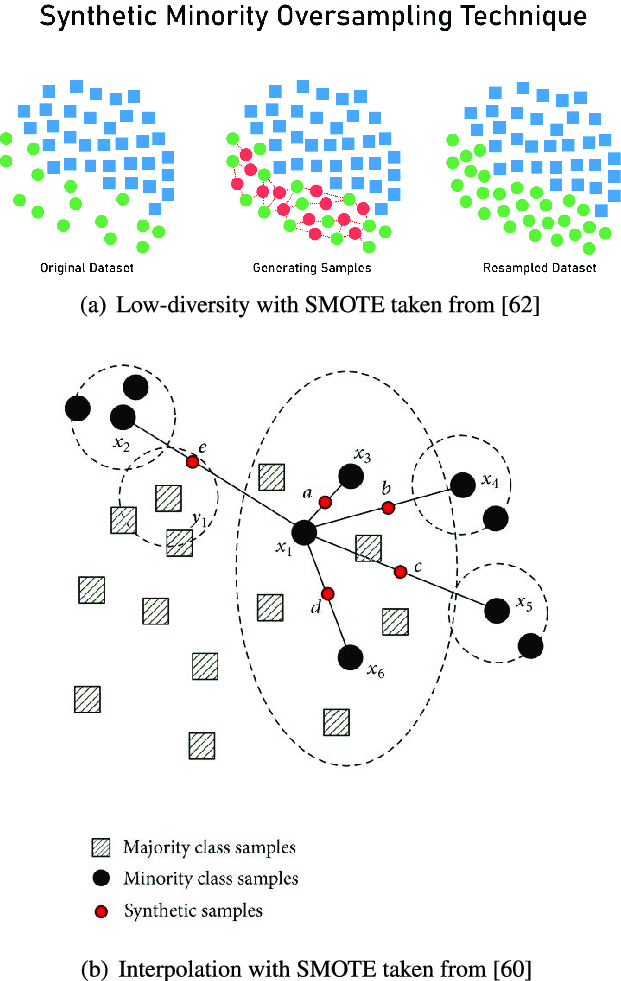
\includegraphics[width=0.8\linewidth]{images/smote_img.png}
        \caption{Smote Illustration taken from~\cite{smoteimg,smoteimg60}}
        \label{fig:smote_img}
    \end{figure}
    
    In many real-world datasets, especially in classification problems, the distribution of classes is often imbalanced, meaning that one class significantly outnumbers the others. This can lead to biased models that perform poorly on minority classes since they have less representation in the data.
    
    SMOTE, which stands for Synthetic Minority Over-sampling Technique~\cite{smote}, is a method used to address imbalanced datasets by generating synthetic samples for the minority class. By doing so, it aims to balance the class distribution and improve the performance of classifiers, particularly in scenarios where the minority class is underrepresented.
    
    \textbf{The SMOTE algorithm:} SMOTE works by creating synthetic instances of minority class samples. Here's a step-by-step explanation of the algorithm:

    \begin{enumerate}
        \item \textbf{Selecting a Minority Instance:} SMOTE starts by randomly selecting a minority instance from the dataset.
        \item \textbf{Finding k-Nearest Neighbors:} Once a minority instance is chosen, SMOTE identifies its k nearest neighbors in the feature space. The value of $k$ is a parameter set by the user.
        \item \textbf{Generating Synthetic Samples:} SMOTE generates synthetic samples by interpolating between the chosen minority instance and its nearest neighbours. For each feature, SMOTE randomly selects a value within the range defined by the feature values of the instance and its neighbours.
        \item \textbf{Adding Synthetic Samples:} The newly generated synthetic samples are added to the dataset, effectively increasing the representation of the minority class.
    \end{enumerate}
    
    By repeating this process for multiple minority instances, SMOTE helps to balance the class distribution and mitigate the issues associated with imbalanced data.